\documentclass[a4paper, 11pt]{article}
\usepackage[portuguese]{babel}
\usepackage[utf8]{inputenc}
\usepackage{indentfirst}
\usepackage{graphicx}
\usepackage{verbatim}
\usepackage{hyperref}
\usepackage{fancyhdr}
\usepackage{listings}
\usepackage{color}
\usepackage[T1]{fontenc}
\usepackage{float}

\pagestyle{fancy}
\renewcommand{\headrulewidth}{0pt}
\lhead{}
\chead{}
\rhead{}
\lfoot{}
\cfoot{\thepage}
\rfoot{}

\begin{document}

\setlength{\textwidth}{16cm}
\setlength{\textheight}{22cm}

\title{
\huge\textbf{Relatório}\linebreak\linebreak
\Huge\textbf{Trabalho Laboratorial 2}\linebreak\linebreak
\linebreak\linebreak
\centering \includegraphics[scale=0.1]{images/feup-logo.png}\linebreak\linebreak
\linebreak
\large Mestrado Integrado em Engenharia Informática e Computação \linebreak\linebreak
\Large{Redes de Computadores}\linebreak
}

\author{\textbf{3MIEIC06 - Bancada 2}\\
\linebreak\\
Miguel Carvalho - \textbf{up201605757} \\
Sandro Campos - \textbf{up201605947} \\
Tiago Cardoso - \textbf{up201605762} \\
\linebreak\linebreak \\
 \\ Faculdade de Engenharia da Universidade do Porto \\ Rua Roberto Frias, s\/n, 4200-465 Porto, Portugal \linebreak\linebreak
\linebreak\linebreak\vspace{1cm}}

\maketitle
\thispagestyle{empty}

\newpage

\tableofcontents 

\newpage

% Sumário
\section{Sumário}
\normalsize 

O presente relatório, realizado no âmbito da unidade curricular de Redes de Computadores, aborda a realização de um trabalho laboratorial com a finalidade de configurar e estudar uma rede de computadores como suporte para o desenvolvimento de uma aplicação de \textit{download}. Esta mesma aplicação permite realizar a transferência de um qualquer ficheiro a partir de um servidor FTP - \textit{File Transfer Protocol}, conhecido o seu URL - \textit{Uniform Resource Locator}.

%1. Introdução
\section{Introdução}

O objetivo deste trabalho é a implementação de uma aplicação que possa fazer uso de uma rede de computadores previamente configurada, e com este relatório pretende-se efetuar uma análise aprofundada de todo esse processo. Segue-se a sua estrutura:
\begin{itemize}
	\item \textbf{Arquitetura} - apresentação dos blocos funcionais.
	\item \textbf{Estrutura do código} - exposição da \textit{API}, principais funções, estruturas de dados e a sua relação com a arquitetura escolhida.
	\item \textbf{Casos de uso principais} - identificação e demonstração da invocação do programa.
	\item \textbf{Validação} - descrição dos testes efetuados à aplicação.
	\item \textbf{Experiências laboratoriais} - descrição e análise sumária de cada uma das experiências realizadas em contexto de laboratório.
	\item \textbf{Conclusões} - síntese da informação apresentada e reflexão acerca dos objetivos de aprendizagem alcançados.
\end{itemize}
%\pagebreak

% Parte 1 - Aplicação
\section{Parte 1 - Aplicação de \textit{download}}

A primeira parte deste trabalho consiste no desenvolvimento de uma aplicação de \textit{download} recorrendo à linguagem de programação C, fazendo uso de \textit{sockets} a partir de ligações TCP - \textit{Transmission Control Protocol}. Para tal houve necessidade de ter em consideração o funcionamento do protocolo FTP, e de estudar algumas das suas normas, como as descritas nos RFC959 e RFC1738, referentes ao processamento de endereços URL.

%2.Arquitetura
\subsection{Arquitetura}

Neste trabalho consideram-se existir dois blocos funcionais, o responsável pelo \textit{parsing} do URL, argumento que se encontra no formato RFC1738\\
\textbf{ftp://<user>:<password>@<host>/<url-path>}, e o que interage com o servidor FTP, desencadeando a transferência do ficheiro pretendido.

%3.Estrutura do código
\subsection{Estrutura do Código}

De acordo com o modelo arquitetural definido, seguem-se as principais funções e estruturas de dados referentes a cada bloco funcional.\linebreak

Para processamento do URL as funções mais relevantes são a \textit{\textbf{parseURL}}, que efetua o \textit{parsing} de cada um dos parâmetros passados através da linha de comandos, e a função auxiliar \textit{\textbf{parseFilename}}, responsável por extrair o nome do ficheiro através do seu caminho relativo no servidor.

O \textit{parsing} encontra-se implementado por uma máquina de estados do tipo \textit{URLstate}, com nomes correspondentes aos elementos relevantes do endereço.

\begin{lstlisting}[language=C]
/**
 * States for the URL parsing state machine  
 */
typedef enum {INIT,FTP,USER,PWD,HOST,PATH} URLstate;
\end{lstlisting}

Estes elementos, após processados, são guardados em variáveis de uma \textit{struct} do tipo \textbf{URLarguments}, cuja declaração se apresenta abaixo.

\begin{lstlisting}[language=C]
/**
 * Arguments obtained from the URL
 */
typedef struct URLarguments
{
  char user[256];
  char pwd[256];
  char hostname[256];
  char filepath[256];
  char filename[256];
  char hostIp[256];
} URLarguments;
\end{lstlisting}

No caso do bloco funcional relativo ao cliente TCP, as funções de maior importância são a \textit{\textbf{openSocket}}, \textit{\textbf{sendCmd}} e \textit{\textbf{receiveResponse}}.

A primeira tem como objetivo criar um \textit{socket} para comunicação com um servidor, dado o seu endereço IP e a porta à qual se conectar. Note-se que a porta para comunicação de controlo a um servidor com protocolo FTP é, por \textit{default}, a nº 21.

A segunda, fazendo uso da ligação estabelecida ao servidor por meio de um \textit{socket} de controlo, escreve comandos para serem recebidos e interpretados pelo mesmo.

A última recebe, por meio desse mesmo \textit{socket}, informação relativa ao envio de um determinado comando para o servidor, um código de 3 dígitos e uma mensagem. Este código pode ser de vários tipos, destacando-se os de ação solicitada concluída com \textbf{êxito (2xx)}, os de ação solicitada a realizar após envio de \textbf{informação complementar}, como uma palavra-passe, \textbf{(3xx)}, e aqueles em que a ação solicitada foi \textbf{rejeitada (4xx e 5xx)}.
Este tipo de informação, também processada através de uma máquina de estados, é guardada em estruturas do tipo \textbf{ServerResponse} como a declarada a seguir.

\begin{lstlisting}[language=C]
/**
 * Server response code and message
 */
typedef struct ServerResponse
{
  char code[4];
  char msg[1024];
} ServerResponse;
\end{lstlisting}

Para se iniciar a transferência do ficheiro é ainda necessário autenticar o utilizador, mudar para o diretório correto, entrar em modo passivo, e requerer o ficheiro ao servidor. Este é posteriormente enviado através de um \textit{socket} de dados criado pelo cliente, e que se encontra conectado a uma porta do servidor atribuída para esse efeito. As funções que intervêm neste processo são a \textit{\textbf{login}}, \textit{\textbf{changeDir}}, \textit{\textbf{enterPasvMode}}, \textit{\textbf{openDataConnection}} e \textit{\textbf{transferFile}}, respetivamente.

%4. Casos de uso principais
\subsection{Casos de uso principais}

De forma a interagir com o programa o utilizador deve recorrer à interface existente da linha de comandos, caso de uso que é único.

Para dar início à aplicação deve então proceder-se à inserção de um só argumento, o URL de um ficheiro num servidor FTP \textit{online}, que vai ser utilizado para transferência. Segue-se um exemplo com a sintaxe a usar:

\begin{lstlisting}[language=C]
./download ftp://<user>:<password>@<host>/<url-path>
\end{lstlisting}

%6. Validação
\subsection{Validação}

A aplicação foi executada com ficheiros de diversas extensões e tamanhos, alojados em servidores distintos, e o comportamento foi o esperado. No terminal podem verificar-se as interações de comunicação existentes entre o cliente e o servidor, como observável na figura 1, em anexo I.

%\pagebreak

%Parte 2 - Experiências
\section{Parte 2 - Configuração e análise da rede}

% Exp1
\subsection{Experiência 1 - Configurar uma rede IP}

Na primeira experiência iniciou-se a configuração de uma rede, conectando duas máquinas, tux1 e tux4, a um \textit{switch}, de forma a possibilitar a comunicação entre elas. Para isso conectaram-se as interfaces eth0 de cada uma ao \textit{switch}, e configuraram-se os seus endereços IP, através do uso do comando \textit{\textbf{ifconfig}}. A sua utilização pode ser observada nos dois comandos iniciais de cada script, em anexo II.

Ao executar o comando \textit{ping} observa-se a troca de \textbf{pacotes ARP}, os de pedido, que são enviados de forma a requerer o \textbf{endereço MAC} da máquina com um determinado \textbf{endereço IP} a alcançar, e os correspondentes de resposta. Os endereços MAC e IP de origem de um pacote ARP correspondem ao sistema que o enviou e de destino os correspondentes no sistema a alcançar. Neste caso, o endereço MAC no pacote de destino é desconhecido, pelo que se questiona a rede acerca da máquina com o IP desejado e espera-se que essa mesma responda com o endereço MAC pretendido, que é posteriormente registado. Em anexo I, na figura 2, segue um exemplo da execução do comando \textit{ping}, e na figura 6, um exemplo de troca de pacotes ARP.

Os diversos tipos de pacote que circulam na rede são distinguidos através de um processo de \textbf{desmultiplexagem}, que permite obter o cabeçalho de uma trama, e identificar o protocolo único a esta associado.

Existe ainda uma interface de rede virtual designada por \textit{\textbf{loopback}}, que cada máquina utiliza para comunicar consigo mesma, de forma a efetuar testes de software e de diagnóstico de conectividade. Observe-se a figura 3, em anexo I.

% Exp2
\subsection{Experiência 2 - Implementar duas \textit{LAN}s virtuais num \textit{switch}}

Nesta experiência implementaram-se duas redes locais virtuais no \textit{switch}, uma englobando as máquinas configuradas na experiência anterior, a vlan20, e a outra contendo o tux22, a vlan21.

O processo de criação e configuração de portas do \textit{switch} a associar a cada uma das \textit{VLANs} encontra-se em anexo II, no registo 1. Para o realizar conectou-se a porta de série de um dos tux's disponíveis a uma das portas deste dispositivo, e invocaram-se os comandos suprareferidos através do \textbf{GTKTerm}. 

Posto isto, e em concordância com os registos guardados, observa-se a existência de dois domínios distintos de \textit{broadcast}, uma vez que a execução do comando \textit{ping -b}, a partir de um qualquer tux, não origina respostas de todas as máquinas configuradas.

% Exp3
\subsection{Experiência 3 - Configurar um router em \textit{Linux}}

O objetivo desta experiência esteve associada com a configuração do tux4 de forma a que este se comportasse como um router, estabelecendo uma conexão entre as \textit{VLAN}s criadas anteriormente.
Para isso houve necessidade de conectar a interface eth1 dessa mesma máquina à vlan21, sub-rede onde se encontrava já presente o tux2. De forma a concluir este processo adicionaram-se ainda duas rotas, uma ao tux1 e outra ao tux4, indicando os endereços IP para reencaminhamento dos pacotes provenientes de cada uma destas máquinas, ativou-se o reencaminhamento de IPs e desativou-se respostas ICMP a \textit{pings broadcast}.
No final já foi possível efetuar comunicação entre os computadores, situação observável, por exemplo, através da execução do comando \textit{ping}. Seguem em anexo I, nas figuras 4 e 5, as tabelas de \textit{forwarding} para o tux21 e para o tux22. Nestas podemos observar, entre outros, parâmetros indicando o destino da rota, \textbf{Destination}, o IP do nó da rede por onde passa a rota, \textbf{Gateway}, e a interface de rede do tux responsável por essa mesma \textit{gateway}, eth0 ou eth1.

Através do programa Wireshark consegue-se observar a troca de pacotes existentes entre os tux, como os ARP e os ICMP. Estes últimos possibilitam testar e efetuar um controlo da rede, enviando pacotes \textbf{Reply}, se o host é alcançável, \textbf{Host Unreachable} caso contrário. Em anexo I, na figura 6, existe um registo ilustrando a troca de pacotes ARP e ICMP. 

% Exp4
\subsection{Experiência 4 - Configurar um router comercial e implementar NAT} 

O objetivo desta experiência esteve relacionado com a configuração de um router comercial e com a implementação da funcionalidade NAT - \textit{Network Address Translation} ao mesmo. 

Para configurar o router comercial adicionaram-se, como segue em anexo II nos scripts individuais, as rotas \textit{default} para cada um dos tux. O tux22 e o tux24 possuem como rota \textit{default} o router comercial configurado na sua rede virtual local, enquanto que o tux21, possui como rota \textit{default} o tux24. A partir deste momento o tux21 é capaz de alcançar qualquer interface da rede, inclusivé a do router. Em anexo I, na figura 7, observa-se um \textit{ping} realizado ao router.

Na iteração seguinte, ao implementar a funcionalidade \textit{NAT}, os endereços privados são convertidos em endereços públicos, recorrendo a tabelas \textit{hash}, e a rede configurada passa a poder comunicar com redes externas. O processo de configuração apresenta-se em anexo I, na figura 8.

Após todo este processo, e para testar a correta configuração das rotas na rede, realizou-se um \textit{ping} ao router a partir do tux21. Observou-se, como seria de esperar, que os pacotes de resposta enviados ao tux21 foram reencaminhados pelo tux24.

% Exp5
\subsection{Experiência 5 - DNS}

Na penúltima experiência, e para concluir a configuração de acesso à internet, configurou-se o serviço de DNS - \textit{Domain Name System} - em cada uma das máquinas. Este tipo de servidor tem como função traduzir cada \textit{hostname} para o seu respetivo endereço IP externo. 

Esta configuração está em todas as máquinas presente no ficheiro '/etc/resolv.conf', e deve conter informação acerca do servidor DNS a aceder cada vez que se pretende contactar com um \textit{hostname} de IP desconhecido, presente na internet. Para isso executaram-se as dois últimos comandos presentes em cada um dos scripts, presentes em anexo II.

Em anexo I, na figura 9, observa-se a troca de \textbf{pacotes DNS} que ocorre quando se efetua \textit{ping} a 'google.com'. O pacote de pedido transporta parâmetros como o nome do \textit{host} e o tempo de vida do pedido, enquanto que a resposta devolve
o endereço IP do \textit{host} requerido e o tempo de vida da resposta.

% Exp6
\subsection{Experiência 6 - Ligações  TCP}
 
Para concluir, na última experiência procurou-se testar a aplicação desenvolvida sob a rede configurada, verificando-se o esperado comportamento do protocolo TCP. Um exemplo de execução da aplicação encontra-se na figura 1, em anexo I.

Durante a execução do programa observa-se o estabelecimento de duas ligações TCP ao servidor FTP. Enquanto uma destas possui a finalidade de trocar de \textbf{mensagens de controlo} entre os intervenientes, a outra permite o envio de \textbf{dados} para o cliente, por parte do servidor. Após terminada a sua função, cada uma destas conexões é devidamente encerrada. Em anexo I, nas figuras 10 e 11, observamos registos Wireshark ilustrando o referido anteriormente.

O protocolo TCP funciona de acordo com o mecanismo \textbf{Selective Repeat ARQ} - \textit{Automatic Repeat Request}, semelhante ao Go-Back-N ARQ, efetuando no entanto o processamento de frames mesmo quando ocorre uma falha na receção. Neste caso, os frames perdidos identificados pelo recetor através do uso de um \textit{acknowledgement number}, são requeridos ao emissor e por este posteriormente enviados. A gama de pacotes que o recetor pode receber a cada momento depende, por isso, da quantidade de pacotes com falha de receção ainda não repostos pelo emissor - \textbf{método da janela deslizante}.

Além disso, durante a transferência de um ficheiro o fluxo de dados depende, a cada momento, do número de ligações TCP que o servidor necessita de servir. Assim sendo, observa-se que quando a rede se encontra mais congestionada, menor é a taxa de transmissão, consequência do servidor distribuir de igual forma a taxa de transferência por cada uma das ligações. 

%9. Conclusões
\section{Conclusões}

A configuração e análise de rede proposta a propósito deste trabalho proporcionou uma maior compreensão dos conceitos abordados de forma teórica nas aulas da unidade curricular. 

Posteriormente, com o desenvolvimento da aplicação de \textit{download}, houve ainda a oportunidade de melhor explorar o funcionamento dos protocolos TCP/IP e FTP, beneficiando de todo o conhecimento técnico que daí advém.

De acordo com o guião fornecido consideramos que os objetivos deste trabalho foram alcançados, dando-o, portanto, por bem sucedido.


% Referências
\begin{thebibliography}{1}
  \bibitem{notes} Manuel P. Ricardo {\em Lab 2 - Computer Networks.} 2018.
\end{thebibliography}

\newenvironment{changemargin}[2]{%
\begin{list}{}{%
\setlength{\topsep}{0pt}%
\setlength{\leftmargin}{#1}%
\setlength{\rightmargin}{#2}%
\setlength{\listparindent}{\parindent}%
\setlength{\itemindent}{\parindent}%
\setlength{\parsep}{\parskip}%
}%
\item[]}{
\end{list}}

% Anexo I - Imagens
\newpage
\section{Anexo I - Imagens}

\begin{figure}[H]
\centering
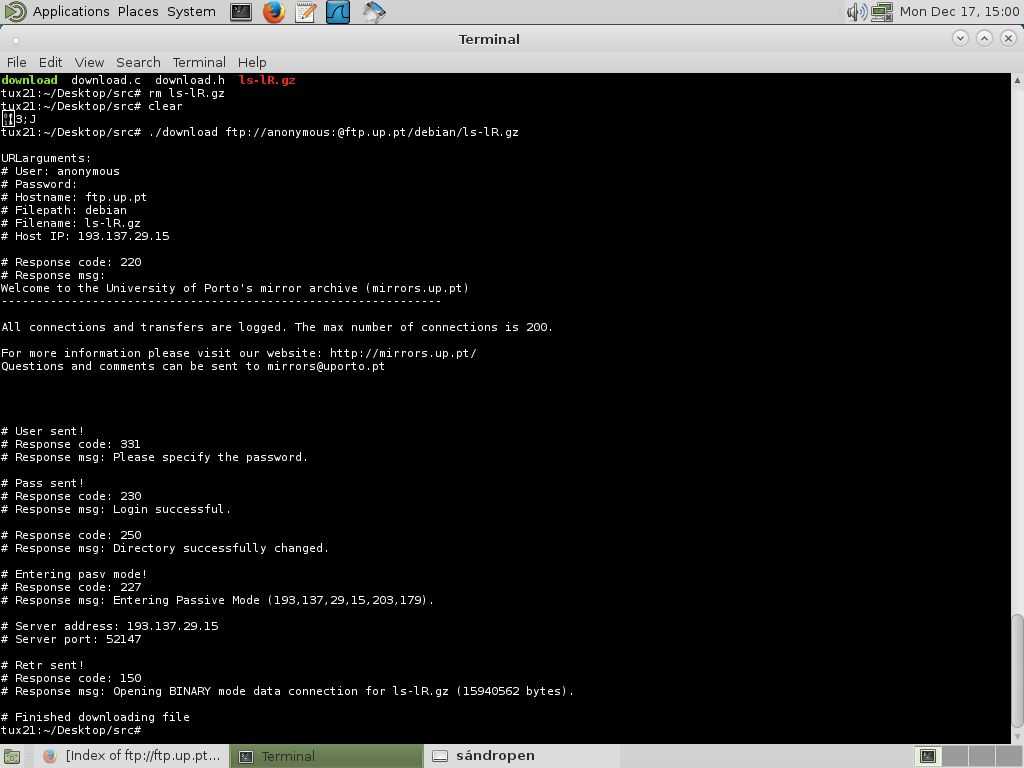
\includegraphics[scale=0.50]{images/exp6_download.png}
\caption{Exemplo de execução da aplicação.}
\end{figure}

\hfill

% exp1
\begin{figure}[ht]
\centering
\includegraphics[scale=0.45]{images/exp1_ping.png}
\caption{Exemplo de execução do comando ping.}
\end{figure}

\hfill

\begin{figure}[H]
\centering
\includegraphics[scale=0.4]{images/exp1_loopback.png}
\caption{Rotina de \textit{loopback} em execução.}
\end{figure}

\hfill

% exp3
\begin{figure}[H]
\centering
\includegraphics[scale=0.5]{images/exp3_tux21.png}
\caption{Rotas no tux21.}
\end{figure}

\hfill

\begin{figure}[H]
\centering
\includegraphics[scale=0.5]{images/exp3_tux22.png}
\caption{Rotas no tux22.}
\end{figure}

\hfill

%exp4
\begin{figure}[H]
\centering
\includegraphics[scale=0.30]{images/exp3_packets.png}
\caption{Troca de pacotes ARP e ICMP.}
\end{figure}

\hfill

\begin{figure}[H]
\centering
\includegraphics[scale=0.50]{images/exp4_pingRouter.png}
\caption{Execução de \textit{ping} ao router.}
\end{figure}

\hfill

%exp5
\begin{figure}[H]
\centering
\includegraphics[scale=0.70]{images/exp4_nat.png}
\caption{Comandos para implementação de \textit{NAT} num router \textit{CISCO}.}
\end{figure}

\hfill

\begin{figure}[H]
\centering
\includegraphics[scale=0.40]{images/exp5_dns.png}
\caption{Troca de pacotes DNS.}
\end{figure}

\hfill

\begin{figure}[H]
\centering
\includegraphics[scale=0.40]{images/exp6_tcpftp.png}
\caption{Exemplo de envio de pacotes de controlo.}
\end{figure}

\hfill

\begin{figure}[H]
\centering
\includegraphics[scale=0.40]{images/exp6_tcpftp2.png}
\caption{Exemplo de envio de pacotes de dados.}
\end{figure}

\clearpage

\newpage
\section{Anexo II - \textit{Scripts} e comandos de configuração}

\begin{changemargin}{-3cm}{-4cm}
{\underline{\textbf{Registo 1 - Criação e configuração de uma \textit{VLAN}}}}
{\small\lstinputlisting{scripts/exp2_vlan}}
\end{changemargin}

\hfill

\begin{changemargin}{-3cm}{-4cm}
{\underline{\textbf{tux21.sh}}}
{\small\lstinputlisting[language=sh]{scripts/tux21.sh}}
\end{changemargin}

\hfill

\begin{changemargin}{-3cm}{-4cm}
{\underline{\textbf{tux22.sh}}}
{\small\lstinputlisting[language=sh]{scripts/tux22.sh}}
\end{changemargin}

\hfill

\begin{changemargin}{-3cm}{-4cm}
{\underline{\textbf{tux24.sh}}}
{\small\lstinputlisting[language=sh]{scripts/tux24.sh}}
\end{changemargin}

\clearpage

% Anexo II
\newpage
\section{Anexo III - Código fonte}

\begin{changemargin}{-3cm}{-4cm}
{\underline{\textbf{download.h}}}
{\small\lstinputlisting[language=C]{src/download.h}}
\end{changemargin}

\hfill

\begin{changemargin}{-3cm}{-4cm}
{\underline{\textbf{download.c}}}
{\small\lstinputlisting[language=C]{src/download.c}}
\end{changemargin}

\end{document}
